% Template for Cogsci submission with R Markdown

% Stuff changed from original Markdown PLOS Template
\documentclass[10pt, letterpaper]{article}

\usepackage{cogsci}
\usepackage{pslatex}
\usepackage{float}
\usepackage{caption}

% amsmath package, useful for mathematical formulas
\usepackage{amsmath}

% amssymb package, useful for mathematical symbols
\usepackage{amssymb}

% hyperref package, useful for hyperlinks
\usepackage{hyperref}

% graphicx package, useful for including eps and pdf graphics
% include graphics with the command \includegraphics
\usepackage{graphicx}

% Sweave(-like)
\usepackage{fancyvrb}
\DefineVerbatimEnvironment{Sinput}{Verbatim}{fontshape=sl}
\DefineVerbatimEnvironment{Soutput}{Verbatim}{}
\DefineVerbatimEnvironment{Scode}{Verbatim}{fontshape=sl}
\newenvironment{Schunk}{}{}
\DefineVerbatimEnvironment{Code}{Verbatim}{}
\DefineVerbatimEnvironment{CodeInput}{Verbatim}{fontshape=sl}
\DefineVerbatimEnvironment{CodeOutput}{Verbatim}{}
\newenvironment{CodeChunk}{}{}

% cite package, to clean up citations in the main text. Do not remove.
\usepackage{apacite}

% KM added 1/4/18 to allow control of blind submission


\usepackage{color}

% Use doublespacing - comment out for single spacing
%\usepackage{setspace}
%\doublespacing


% % Text layout
% \topmargin 0.0cm
% \oddsidemargin 0.5cm
% \evensidemargin 0.5cm
% \textwidth 16cm
% \textheight 21cm

\title{Sticks, leaves, buckets, and bowls: Distributional patterns of
children's at-home object handling in two subsistence societies}

\usepackage{booktabs}
\usepackage{longtable}
\usepackage{array}
\usepackage{multirow}
\usepackage{wrapfig}
\usepackage{float}
\usepackage{colortbl}
\usepackage{pdflscape}
\usepackage{tabu}
\usepackage{threeparttable}
\usepackage{threeparttablex}
\usepackage[normalem]{ulem}
\usepackage{makecell}
\usepackage{xcolor}

\author{Kennedy Casey \\
        University of Chicago \\
        \texttt{\small{kbcasey@uchicago.edu}}
\And \textbf{Mary Elliott} \\
             University of Texas at Dallas \\
             \texttt{\small{maryle18@gmail.com}}
\And \textbf{Anapaula Silva Mandujano} \\
             University of Chicago \\
             \texttt{\small{anapaula@uchicago.edu}}   
\And \textbf{Kimberly Shorter} \\
             University of Chicago \\
             \texttt{\small{klshorter@uchicago.edu}}
\AND \textbf{Elizabeth Mickiewicz} \\
             University of Chicago \\
             \texttt{\small{lizmick9@uchicago.edu}}         
\And \textbf{Mara Duquette} \\
             University of Chicago \\
             \texttt{\small{duquettemara@uchicago.edu}}
\And \textbf{Elika Bergelson} \\
             Duke University \\
             \texttt{\small{elika.bergelson@duke.edu}}
\And \textbf{Marisa Casillas} \\
             University of Chicago \\
             \texttt{\small{mcasillas@uchicago.edu}}}

\newlength{\cslhangindent}
\setlength{\cslhangindent}{1.5em}
\newenvironment{CSLReferences}%
  {}%
  {\par}

\begin{document}

\maketitle

\begin{abstract}
Object-centric interactions provide rich learning moments for young
children, including opportunities to discover word meanings. Children's
own object handling, in particular, forms a key source of input -- one
that varies across cultures and across development. Using daylong photo
streams from child-worn cameras, we analyze \textgreater16k images to
identify the frequency and targets of child object handling across the
first four years in two small-scale subsistence farming communities on
opposite sides of the globe (Papuan and Mayan). Overall, we see a
general consistency in the broad composition of handled objects across
cultures and age, likely reflecting stable properties of children's
physical environments and day-to-day routines. However, the exact
objects available to children vary both within and across communities
and also diversify with age. These various distributions of handling
patterns are discussed in their relation to potential consequences for
word learning.

\textbf{Keywords:}
culture; object play; word learning; daylong recording; egocentric
images
\end{abstract}

\hypertarget{introduction}{%
\section{Introduction}\label{introduction}}

The objects that we regularly pick up and handle---a coffee cup, a
laptop, a baby bottle---offer a window into the physical, social, and
cultural contexts that shape our understanding of the world. In this
paper, we take a glimpse into everyday life at its beginnings by
exploring children's at-home object handling from early infancy until
age four.

\hypertarget{object-handling-and-word-learning}{%
\subsection{Object handling and word
learning}\label{object-handling-and-word-learning}}

We contextualize our study with respect to the effects of object-centric
interaction on word learning. For young learners, objects---along with
their associated activities and surrounding language---form a critical
source of input. Caregivers' tendency to use nouns referring to objects
in the here-and-now positively predicts children's early word
comprehension (Bergelson \& Aslin, 2017; see also Slone, Smith, \& Yu,
2019) by helping learners map word forms onto their meanings in and
across real-time interaction (e.g., Yu \& Smith, 2013; Yurovsky, Smith,
\& Yu, 2013). Children also actively shape their own input via the
objects that they choose to pick up and handle. Children's own object
handling influences not only which objects dominate in their visual
fields (Suanda, Barnhart, Smith, \& Yu, 2019) but sometimes also the
language that they hear about those objects (e.g., Chang, Barbaro, \&
Deák, 2016)

How frequently do children engage in object-centric interactions? First,
hands---others' and their own---are in good supply in young children's
view of the world, especially after early infancy (Fausey, Jayaraman, \&
Smith, 2016; Jayaraman, Fausey, \& Smith, 2017; Long, Kachergis,
Agrawal, \& Frank, 2020). Infants' own object handling is relatively
frequent: Herzberg and colleagues (2021) find that US infants handle
objects \({\sim}60\%\) of the time during at-home play, Yu and
colleagues (2013) find \({\sim}70\%\) when including joint handling with
adults in US in-lab object play, and Casillas and Elliott (2021) find
\({\sim}15\) and 17\% object handling in daylong photo streams in a
Papuan and a Mayan community, respectively.

Concurrent with these events, children will sometimes encounter
linguistic information relating to the focused-on object (e.g., its
label and associated concepts). However, this critical additional
ingredient for word learning may only occur during a small subset of
total object handling time. We do not yet know how often objects in the
here-and-now are typically talked about over the course of children's
whole waking days at home, but we do know that such talk fluctuates
across high and low activity periods (Bergelson, Amatuni, Dailey,
Koorathota, \& Tor, 2019). We also know that children's object handling
varies enormously across the first few years due to cross-cultural
differences in available objects and caregiving practices as well as
maturational constraints.

\hypertarget{object-handling-across-cultures}{%
\subsection{Object handling across
cultures}\label{object-handling-across-cultures}}

The array of objects available to children varies in type and prevalence
across cultures. Objects spread via globalization (e.g., plastic bags)
and objects with a basic functional role that arose similarly across
many groups (e.g., spoon-like tools for eating) are likely to appear
widely, while other objects remain specific to people and places (e.g.,
the gourd and bombilla for drinking mate in much of South America,
stemming from Indigenous Guaraní and Tupí tradition).

Early access to objects is also shaped by culture-specific practices for
carrying children, keeping them safe and warm, and scaffolding the
development of locally-valued capacities (e.g., word learning in many US
families, walking in Kenyan Kipsigis families: Super, 1976; see Adolph,
Karasik, \& Tamis-LeMonda, 2010, for an overview). Take, for example,
middle-class US family homes, which have been noted for their large
quantities of possessions (``clutter''), much of which is designed
specifically for children (e.g., toys and children's books: Arnold,
Graesch, Ochs, \& Ragazzini, 2012). We might infer, based on these
assemblages of home objects, that much of what children do and talk
about at home is centered around what particularly interests them.
Recent work by Herzberg and colleagues (2021) underscores this point
with data from infants (13--23 months old) who spent nearly 70\% of
their time in object play with toys or a mix of toys and non-toys, with
\({\sim}100\%\) of infants playing with children's books and stuffed
animals, and a total of 32 toy types appearing in \({\ge}25\%\) of
infants' play. Non-toy play was also common but still appeared to
predominantly include infant-specific objects (e.g., sippy cups, baby
spoons, high chairs, pacifiers). We would expect many of these items to
be rare in other parts of the world, with much greater overlap between
objects for infants and objects for adults (e.g., Karasik, Schneider,
Kuchirko, \& Tamis-LeMonda, 2018).

\hypertarget{object-handling-across-age}{%
\subsection{Object handling across
age}\label{object-handling-across-age}}

In early infancy, children have little ability to hold things or to
control their posture, primarily experiencing objects through what
others bring near to them. Faces, rather than objects, may make up a
much greater proportion of their social and visual input early on
(Fausey, Jayaraman, \& Smith, 2016; Jayaraman, Fausey, \& Smith, 2017;
but see also Long, Kachergis, Agrawal, \& Frank, 2020). However, later
gains in manual dexterity and gross motor skill (e.g., sitting,
crawling, walking) increasingly widen children's ability to seek, reach,
and grab a diversity of objects in their environments. Increasing motor
development not only gives children greater control over what objects
they handle, but also \emph{how} they elicit social information relating
to objects and for how long (Adolph, Karasik, \& Tamis-LeMonda, 2010;
Gaskins, 2000; Herzberg, Fletcher, Schatz, \& Tamis-LeMonda, 2021;
Kretch, Franchak, \& Adolph, 2014; Sanchez, Long, Kraus, \& Frank,
2018).

\hypertarget{the-current-study}{%
\subsection{The current study}\label{the-current-study}}

Overall, while prior work makes a strong case for the impact of
children's object-centric interactions on their word learning, the
findings: (a) are limited to a culturally narrow sample of populations,
(b) have tended to rely on short recordings that limit the scope of
object-centered interactions analyzed, and (c) have rarely examined in
detail the distributions of individual objects that children typically
interact with at home (exceptions include Bergelson, Amatuni, Dailey,
Koorathota, \& Tor, 2019; Casillas \& Elliott, 2021; Herzberg, Fletcher,
Schatz, \& Tamis-LeMonda, 2021).

In the current work, we use daylong photo streams from child-worn
cameras to analyze object handling by children under age four in two
rural, small-scale subsistence farming communities on opposite sides of
the globe: Rossel Island (``Rossel''; Milne Bay Province, Papua New
Guinea) and Tenejapa (``Tseltal''; Chiapas, Mexico). While these
communities are comparable in many ways (e.g., rural, swidden
horticulturalist, housed in multi-generation family complexes), prior
work has established substantial differences in the organization of
young children's daily lives, child carrying practices, and each
community's level of market integration (i.e., greater availability of
synthetic materials in Tenejapa), leading us to expect differences in
the objects that children handle across the day and early lifespan
(Brown \& Casillas, 2021; Casillas, Brown, \& Levinson, 2020, 2021;
Casillas \& Elliott, 2021).

Using these manually annotated photo streams, we first establish how
often children handle objects from different categories (e.g., food
vs.~tools), both by the total amount of handling and by number of unique
objects per hour in each category across sites. We explore the top
individual objects in each site along with the overlap that exists
between sites. We then investigate how the rate and characteristics of
object handling change with age.

Our findings reveal relative consistency in the broad composition of
objects handled by children, both between sites and across age, with a
few important exceptions: a greater diversity of synthetic objects
handled by Tseltal children (e.g., relating to greater market
integration), more time spent with immovable objects for Rossel children
(e.g., relating to socializing time on/near household verandas), and a
greater diversity of held objects and greater number of transitions
between handled objects across age. While we focus here on describing
the distributional patterns of children's object handling, we do this
with an eye toward the cognitive and linguistic implications of these
experiences---namely, consequences for word learning.

\hypertarget{method}{%
\section{Method}\label{method}}

\hypertarget{corpus}{%
\subsection{Corpus}\label{corpus}}

Daylong photo streams consisted of images captured approximately every
15 (Rossel) to 30 (Tseltal) seconds over the course of 8 (Rossel) to 9
(Tseltal) waking hours at home. Children wore a recording vest equipped
with a camera (Narrative Clip 1) and miniature fisheye lens (Photojojo
Super Fisheye) that provided a 180\(\text{\textdegree}\) view of the
environment. For younger infants who were not yet walking, the camera
was instead worn by the primary caregiver. Previously, 83 daylong photo
streams (113,668 photos) had been comprehensively manually annotated for
the presence or absence of child object handling (Casillas \& Elliott,
2021). Here, we further annotate and analyze the subset of 16,916 with
confirmed child object handling in the present study.

We included one randomly selected daylong photo stream from each of 77
children with object handling in the original data set (Rossel: 41,
Tseltal: 36). One participant had no usable images (see below for
exclusion information), so our analyses are based on 76 photo streams.
Children ranged in age from 0 to 48 months
(\emph{M}\textsubscript{\emph{Rossel}} = 21.9,
\emph{M}\textsubscript{\emph{Tseltal}} = 22.7). The amount of object
handling and thus the number of photos available to be annotated varied
across children, ranging from 1 to 631
(\emph{M}\textsubscript{\emph{Rossel}} = 238.2,
\emph{M}\textsubscript{\emph{Tseltal}} = 198.6).

\begin{CodeChunk}
\begin{figure}[h]

{\centering \includegraphics{figs/examples-fig-1} 

}

\caption[Example images with object and category labels]{Example images with object and category labels.}\label{fig:examples-fig}
\end{figure}
\end{CodeChunk}

\hypertarget{manual-annotation}{%
\subsection{Manual annotation}\label{manual-annotation}}

Photos were annotated with IMCO, an open-source Python program adapted
for efficient coding of photo streams (Casey, Fisher, Tice, \& Casillas,
2022). Annotators provided labels for the handled object(s) in each
photo (e.g., ``stick'') and selected among a set of predefined
categories to characterize each type of object (e.g., ``Natural'').
Categories included consumables (``Food''; food, drinks, and drugs),
mealtime tools (``Tool-M''), toys, clothing, tools for working \emph{or}
cleaning (``Tool-W''), large or immovable objects (e.g., furniture and
housing structures), natural objects, and miscellaneous synthetic
objects (see Figure 1 for example images and Table 1 for example objects
from each category). In the reported findings, ``object'' refers to any
exemplar of a type of object (e.g., any stick) rather than a particular
instance of an object (e.g., a specific stick), and ``object category''
refers to the predefined categories we used for each object type (e.g.,
``Natural,'' ``Toy,'' ``Immovable'').

\hypertarget{data-preparation-and-reliability}{%
\subsection{Data preparation and
reliability}\label{data-preparation-and-reliability}}

Images were excluded if they were too dark, bright, blurry, or covered
for annotators to identify handled objects, if annotators were otherwise
unsure about what objects were being handled, if there was no handled
object, or if the researcher was still present when the image was
captured (\emph{n} = 1,138, or 6.7\% of the data set). To avoid
unnecessary data loss, all excluded photos were checked by at least one
other annotator and re-included for analysis if objects were
identifiable. In total, 15,778 images were deemed usable by annotators
(9,223 for Rossel, 6,555 for Tseltal).

To confirm sufficient reliability, 20\% of photo streams were double
coded. Reliability annotations were equally spread across sites and ages
and included a total of 8,288 images. At the category level, annotators
agreed on 91.2\% of decisions (Rossel: 91.9\%, Tseltal: 90.6\%), on
average across photo streams. At the object label level, annotators
agreed on 85.1\% of decisions (Rossel: 86.1\%, Tseltal: 84.3\%).

\begin{table}[!ht]

\caption{\label{tab:top-objects}Number of unique objects (N) and objects handled by the most children, for each category, across sites.}
\centering
\resizebox{\linewidth}{!}{
\begin{tabular}[t]{lrlrl}
\toprule
\multicolumn{1}{c}{\textbf{ }} & \multicolumn{2}{c}{\textbf{Rossel}} & \multicolumn{2}{c}{\textbf{Tseltal}} \\
\cmidrule(l{3pt}r{3pt}){2-3} \cmidrule(l{3pt}r{3pt}){4-5}
\textbf{Object Category} & \textbf{N} & \textbf{Top Objects} & \textbf{N} & \textbf{Top Objects}\\
\midrule
Food & 38 & betelnut, coconut, tuber & 54 & bean, tortilla, chips\\
Synthetic & 68 & blanket, woven basket, bucket & 68 & blanket, plastic bag, bucket\\
Natural & 21 & stick, leaf, rock & 13 & stick, plant, tree\\
Toy & 21 & ball, book, swing & 42 & toy car, ball, book\\
Mealtime Tool & 21 & bowl, spoon, knife & 11 & bowl, cup, baby bottle\\
Clothing & 16 & shirt, skirt, purse & 21 & shirt, pants, shoe\\
Immovable & 20 & stairs, wall, floor & 19 & chair, door, fence\\
Work Tool & 16 & knife, broom, baby bathtub & 30 & broom, clothesline, embroidery ring\\
\bottomrule
\end{tabular}}
\end{table}

\hypertarget{results}{%
\section{Results}\label{results}}

\hypertarget{overall-frequency-statistics}{%
\subsection{Overall frequency
statistics}\label{overall-frequency-statistics}}

Children handled an average of 26.7 unique objects per day (median =
27.0, \emph{SD} = 16.0, range = 1--58), with no significant differences
across sites (\emph{M}\textsubscript{\emph{Rossel}} = 26.3,
\emph{M}\textsubscript{\emph{Tseltal}} = 27.2, \emph{W} = 700.50,
\emph{p} = 0.863). The distribution of handled objects was highly
right-skewed within and across children. Each child's distribution was
skewed such that a small group of objects was handled in a majority of
their images but most objects were handled for only short periods of
time (Figure 2). Across children, common objects followed a similar
Zipfian distribution: some objects were handled by many children, but
most objects were only handled by 1--2 children in each site (Rossel:
55.7\%, Tseltal: 60.9\%).

Comparing across sites, 34.8\% of objects were handled by both Rossel
and Tseltal children, and several shared objects were among the most
frequently handled in both sites. In fact, among the top 25 most common
objects\footnote{The study camera was the object that was handled by the
  most children in both sites (Rossel: 68.3\%, Tseltal: 91.4\% of
  children; see Bergelson, Amatuni, Dailey, Koorathota, \& Tor, 2019,
  for a similar effect) but accounted for a relatively small percentage
  of each child's object handling time, on average
  (\emph{M}\textsubscript{\emph{Rossel}} = 3.6\%,
  \emph{M}\textsubscript{\emph{Tseltal}} = 6.5\% of images). Inclusion
  of study-related items did not qualitatively change any of the
  reported results, unless otherwise noted}, 10 were shared across sites
(Figure 3).

\begin{CodeChunk}
\begin{figure}[h]

{\centering 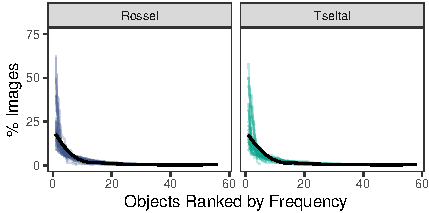
\includegraphics{figs/zipfian-objects-fig-1} 

}

\caption[Zipfian distribution of objects]{Zipfian distribution of objects. For each child, the top object was defined as the object appearing in the greatest number of images; thus, the identity of the top object does not match across all children. Points reflect log-transformed proportion estimates for individual children.}\label{fig:zipfian-objects-fig}
\end{figure}
\end{CodeChunk}

\begin{CodeChunk}
\begin{figure*}[!ht]

{\centering 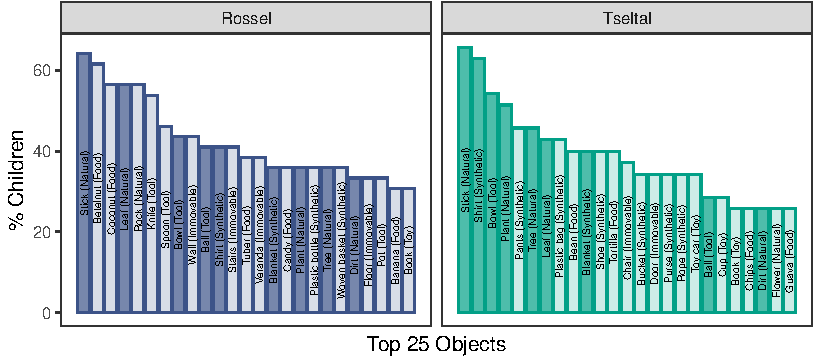
\includegraphics{figs/top-objects-fig-1} 

}

\caption[Non-study-related objects handled at least once by the most children in each site]{Non-study-related objects handled at least once by the most children in each site. Filled bars represent objects that were among the top 25 for both sites.}\label{fig:top-objects-fig}
\end{figure*}
\end{CodeChunk}

We exclude from the following analyses, any hour in which a child did
not handle any objects; inclusion of these cases creates a second mode
at 0, violating our statistical models' assumption of normality.

\hypertarget{effects-of-object-category}{%
\subsection{Effects of object
category}\label{effects-of-object-category}}

We quantified the distribution of object categories at two timescales:
across the whole waking day (i.e., overall \% handling for different
object categories across all images) and across individual hours (i.e.,
number of unique objects from different object categories per hour).

During any given hour, children handled 5.3 objects from 3.0 different
categories, on average (median = 4.0 objects, \emph{SD} = 4.9, range =
0--27). To test for differences across sites and categories, we ran
individual linear mixed-effects regressions for each of the eight object
categories, with category membership dummy coded (i.e., objects
belonging to the target category for a given model = 1, objects
belonging to other categories = 0). Each regression model included fixed
effects of site, category, and a site-by-category interaction as well as
random intercepts for individual children\footnote{lmer(unique
  objects/hour \({\sim}\) category (target/non-target; factorial) * site
  (Rossel/Tseltal; factorial) + (1 \textbar{} child))}. After correcting
for multiple comparisons, we found a significant main effect of the
synthetic object category (\(\beta\) = 0.35, \emph{SE} = 0.09, \emph{t}
= 4.04, \emph{p} = 0.001) and a marginal site-by-synthetic interaction
(\(\beta\) = 0.36, \emph{SE} = 0.12, \emph{t} = 2.93, \emph{p} = 0.058)
such that children handled more unique synthetic objects per hour than
objects from other categories, and this effect was stronger for Tseltal
children than for Rossel children. Additionally, we found negative main
effects for the toy (\(\beta\) = -0.42, \emph{SE} = 0.13, \emph{t} =
-3.14, \emph{p} = 0.034), mealtime tool (\(\beta\) = -0.35, \emph{SE} =
0.12, \emph{t} = -2.96, \emph{p} = 0.056), clothing (\(\beta\) = -0.32,
\emph{SE} = 0.11, \emph{t} = -3.02, \emph{p} = 0.049), and work tool
(\(\beta\) = -0.65, \emph{SE} = 0.17, \emph{t} = -3.86, \emph{p} =
0.002) categories, indicating that children handled fewer unique objects
from these categories per hour relative to other categories. Finally, a
significant main effect of the immovable object category (\(\beta\) =
0.43, \emph{SE} = 0.11, \emph{t} = 3.95, \emph{p} = 0.002) and a
significant site-by-immovable interaction (\(\beta\) = -0.76, \emph{SE}
= 0.17, \emph{t} = -4.44, \emph{p} \textless{} 0.001) revealed that
children handled more unique immovable objects per hour than objects
from other categories, and this effect was stronger for Rossel children
than for Tseltal children (Figure 4).

\begin{CodeChunk}
\begin{figure}[!h]

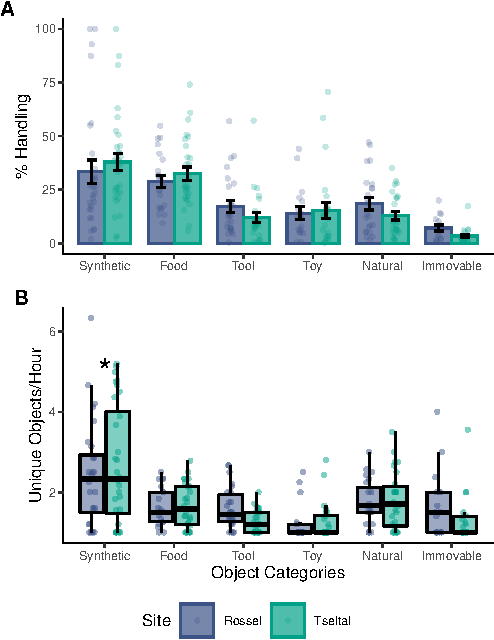
\includegraphics{figs/overall-stats-fig-1} \hfill{}

\caption[Rate of unique objects handled per hour by object category]{Rate of unique objects handled per hour by object category. Points reflect means for individual children across all hours of recording. Asterisks indicate significant differences between sites after correcting for multiple comparisons.}\label{fig:overall-stats-fig}
\end{figure}
\end{CodeChunk}

\hypertarget{effects-of-age}{%
\subsection{Effects of age}\label{effects-of-age}}

Prior work with this same data set indicated a significant increase in
object handling across the first four years (Casillas \& Elliott, 2021).
By adding information about \emph{what} objects children are handling,
we can now explore finer-grained characteristics of age-related change
in object handling. We investigate changes in (a) the distribution of
object categories, (b) the number of unique objects and categories
handled per hour, and (c) transitions between objects and categories per
hour.

\hypertarget{do-children-handle-different-types-of-objects-with-age}{%
\subsubsection{Do children handle different types of objects with
age?}\label{do-children-handle-different-types-of-objects-with-age}}

We fit individual linear regressions predicting the proportion of
handling time for each category as a function of age (in months), site,
and their interaction. We included number of images as an additional
fixed effect to account for the wide range in total available images for
each child (range = 1--631), leading to a greater likelihood of
detecting proportions near 0 or 1 when there were only a handful of
images\footnote{As expected, number of handling images was correlated
  with age (\emph{r} = 0.50 {[}0.31, 0.65{]}, \emph{p} \textless{}
  0.001), which we attribute to changes in motor development and
  permitted object access over the first four years (Casillas \&
  Elliott, 2021)---the correlation is an artifactual outcome of
  development. Including both variables as fixed effects in a regression
  poses no technical issue in estimating \(R^{2}\), but does limit the
  total variance attributed independently to either variable (Wurm \&
  Fisicaro, 2014). Thus, for models of non-proportional measures, we
  rely solely on age to capture this variance (i.e.,
  lmer(non-proportional DV \({\sim}\) age (months; numeric) * site
  (Rossel/Tseltal; factorial) + (1 \textbar{} child)).}. This analysis
revealed no significant age-related changes in the frequency of handling
of different object categories\footnote{The only exception was an
  initial finding of a decrease in handling of clothing over age
  (\(\beta\) \textless{} 0.001, \emph{SE} = 0.00, \emph{t} = -2.88,
  \emph{p} = 0.005). However, after removing study-related clothing
  (i.e., the vest containing the camera), this effect was no longer
  significant.} and no significant site-by-age interaction effects (all
adjusted \emph{p}s \textgreater{} 0.05). Thus, the the broad composition
of handled objects remained largely stable over age.

\hypertarget{does-object-handling-diversify-with-age}{%
\subsubsection{Does object handling diversify with
age?}\label{does-object-handling-diversify-with-age}}

In addition to the overall age-related increase in handling found by
Casillas and Elliott (2021), we see that, with increasing age, children
handled more unique objects per hour (\(\beta\) = 0.12, \emph{SE} =
0.03, \emph{t} = 3.60, \emph{p} = 0.001; Figure 5A) and more objects
from different categories per hour (\(\beta\) = 0.06, \emph{SE} = 0.01,
\emph{t} = 4.45, \emph{p} \textless{} 0.001; Figure 5B). These effects
were consistent across sites; we found no main effects of site or
interactions between site and age (all \emph{p}s \textgreater{} 0.05).

\hypertarget{does-object-handling-become-more-complex-with-age}{%
\subsubsection{Does object handling become more complex with
age?}\label{does-object-handling-become-more-complex-with-age}}

Analysis of children's relative rate of transition between objects per
hour (i.e., the number of transitions from one object to another divided
by the number of available objects for that hour) did not reveal an
overall age-related increase (\(\beta\) = 0.01, \emph{SE} = 0.00,
\emph{t} = 1.59, \emph{p} = 0.116). However, there was a significant
main effect of site (\(\beta\) = -0.30, \emph{SE} = 0.13, \emph{t} =
-2.37, \emph{p} = 0.020; Figure 6C), indicating that Tseltal children
made fewer transitions between objects per hour than Rossel children.
While the site-by-age interaction term did not reach statistical
significance (\(\beta\) = 0.01, \emph{SE} = 0.00, \emph{t} = 1.54,
\emph{p} = 0.128, descriptively, this difference appears to be more
pronounced for younger children. At the category level, we found that
children made marginally more transitions between object categories per
hour with age (\(\beta\) = 0.01, \emph{SE} = 0.01, \emph{t} = 1.69,
\emph{p} = 0.095), in addition to a marginal main effect of site
(\(\beta\) = -0.53, \emph{SE} = 0.31, \emph{t} = -1.70, \emph{p} =
0.092; Figure 6D) that mirrors the finding for object transitions:
Tseltal children made fewer category transitions per hour than Rossel
children.

\begin{CodeChunk}
\begin{figure}[!ht]

{\centering 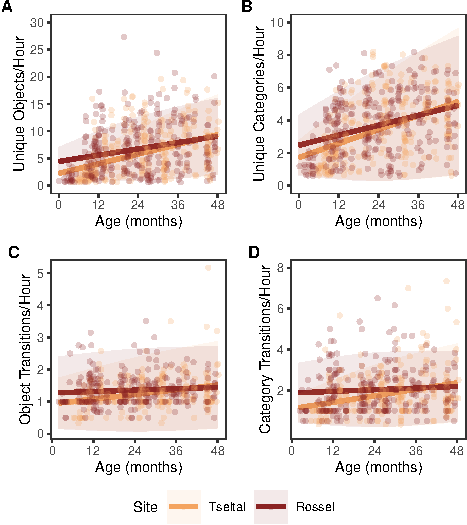
\includegraphics{figs/age-effects-fig-1} 

}

\caption[(A) Unique objects and (B) object categories handled per hour as a function of age]{(A) Unique objects and (B) object categories handled per hour as a function of age. (C) Relative number of transitions between objects and (D) object categories per hour as a function of age. Points reflect raw hourly counts for each child, and lines reflect model predictions with shaded standard error regions.}\label{fig:age-effects-fig}
\end{figure}
\end{CodeChunk}

\hypertarget{discussion}{%
\section{Discussion}\label{discussion}}

We annotated and analyzed 16,916 images of at-home child object handling
from children under age four in two subsistence communities from
opposite sides of the globe. Our main findings are as follows:
Children's overall time spent within categories (e.g., food vs.~natural
vs.~immovable) appears stable across age and cultural context. In
contrast, when it comes to the number of unique objects per hour,
children handled a greater diversity of synthetic and immovable objects,
relative to the other categories, and did so to different extents across
sites. The rate of transition between objects also varied between sites,
with only Tseltal children significantly increasing their transition
rate over age. Finally, time spent with objects is Zipfian-distributed,
and many of the most common objects within site were also common across
the two sites. We discuss this rich set of findings with respect to (a)
object handling as a window into children's worlds in general and (b)
the implications of object handling patterns for word learning.

\hypertarget{objects-as-insight-into-childrens-worlds}{%
\subsection{Objects as insight into children's
worlds}\label{objects-as-insight-into-childrens-worlds}}

These findings, while preliminary, suggest that different measures of
object handling reveal differing aspects of children's worlds. The total
time children spend handling objects of different types (e.g., natural,
immovable, synthetic, etc.) appears stable across age and sites
(consistent with Long, Kachergis, Bhatt, \& Frank, 2021, for visually
present categories). Specifically, food and synthetic objects are most
prevalent. We suggest that this measure of \textbf{total time spent
within categories} may reflect stable properties of children's physical
environments and their routine activities, across age and across diverse
contexts. If we were to sample in other communities, we would expect to
find more differences {[}e.g., more time spent with toys in US
middle-class samples; Herzberg, Fletcher, Schatz, \& Tamis-LeMonda
(2021){]}, but these two rural subsistence communities show overall
similar profiles despite substantial differences in their current market
integration, the organization of daily life, infant carrying practices,
and other aspects of their cultural milieux (Brown \& Casillas, 2021;
Casillas, Brown, \& Levinson, 2020, 2021; Casillas \& Elliott, 2021).

In contrast, the \textbf{number of individual objects} children handle
reveals strong age-related change, as well as some differences between
sites. Children's object handling diversifies within and across
categories as they get older. This means more unique objects handled,
from more categories, and for Tseltal children, more frequent
transitions between objects. Note that this effect may be stronger for
Tseltal children because they are more restricted in their movements
early on, as they are often carried in a sling and therefore less freely
able to seek out and handle new objects (Casillas \& Elliott, 2021).
Compared to other categories, children handle a greater diversity of
synthetic objects (stronger for Tseltal) and immovable objects (stronger
for Rossel) per hour. These cross-site differences reflect the greater
market integration (and hence availability of diverse synthetic objects)
of the Tseltal community and the long daily periods of socializing
around and climbing on family verandas in the Rossel community.

We suggest that the individual objects children handle give us insight
into development. Through identification of the specific objects
children engage with, we can detect age-related changes in object access
along with the dynamics of object-centric interaction (e.g., rate of
transition between objects). Moreover, knowing what objects children
handle can reveal many facets of everyday life that vary across economic
and cultural contexts (e.g., whether a variety of toys is available for
purchase nearby, or daily socializing takes place on climbable
surfaces).

\hypertarget{implications-for-word-learning}{%
\subsection{Implications for word
learning}\label{implications-for-word-learning}}

Our data indicate that children are exposed to a stable and wide variety
of object categories in the first four years of life. Children also have
increasing access to a diversity of objects within categories as they
get older. Similarity in the distribution of categories across sites
suggests some basis for expecting similarity in early object label and
associated word knowledge by children in these two sites. Individual
objects also show a Zipfian distribution in how they are handled, with
some handled frequently and most handled infrequently. This distribution
may help support word learning (see Carvalho, Chen, \& Yu, 2019;
Clerkin, Hart, Rehg, Yu, \& Smith, 2017; Long, Kachergis, Bhatt, \&
Frank, 2021; Montag, Jones, \& Smith, 2018) and, in tandem with other
observed effects across age and cultural context, may indicate which
words (i.e., object names or other object-relevant words) children are
likely to learn first and how their semantic networks grow within and
across categories.

\hypertarget{future-directions}{%
\subsection{Future directions}\label{future-directions}}

In the current work, we grouped objects on the basis of broad semantic
categories. While this categorization allows us to broadly describe the
distribution of handling across different types of objects, it does not
necessarily give us insight into the specific associated activity or
applied function. Knowing more about how objects are being used in
context could help (a) indicate links between social and linguistic
behavior and (b) reveal more changes over developmental time (e.g., a
spoon as a teething toy, musical instrument, and, ultimately, a
utensil).

To more directly compare to existing data from other cultural contexts
also require that we further analyze the temporal characteristics of
handling bouts and track unique object tokens rather than just types
(Herzberg, Fletcher, Schatz, \& Tamis-LeMonda, 2021) We note, however,
that this will be near-impossible for some object types (e.g., leaves,
twigs). Furthermore, we would like to extend our comparison to other
communities, rural and urban, but this will require daylong photo
collection in these other sites. We find less within-site overlap in
exact objects handled by Rossel and Tseltal children compared to
Herzberg, Fletcher, Schatz, \& Tamis-LeMonda (2021)'s US data, but this
may be as much due to recording type (e.g., two-hour videos) as to
cultural difference.

Our most urgent goal is to analyze the speech surrounding bouts of
object handling to derive estimates of how often the objects are talked
about, what is mentioned, and by whom. By combining these daylong photo
streams with audio data in two unrelated cultural contexts, our aim is
to develop a benchmark against which models and mechanisms of word
learning via object-centric interaction can be tested.

\hypertarget{conclusion}{%
\subsection{Conclusion}\label{conclusion}}

Children's material worlds---especially the objects they handle---tell
us what they are interested in, what they do and talk about with others,
what they are allowed to access, and more. Handled objects offer
children a range of sensory experiences that could be paired with the
social, linguistic, and physical information around them. In the present
study we examined coarse patterns in young children's at-home object
handling in two unrelated subsistence communities, finding many striking
similarities despite differences in the communities' market integration
and ways of life. If indeed object-centric interactions guide word
learning and other types of social learning, the present data provide
some basis for kernels of similarity in experience across culture and
change with developmental time. \emph{However}, the current data equally
suggest that any story along those lines must also mention the immense
variation we have begun to unpack in the assemblages of unique objects
handled by individual children, as well as the very \emph{narrow} slices
of time children actually spend with the vast majority of objects.

\hypertarget{references}{%
\section{References}\label{references}}

\setlength{\parindent}{-0.1in} 
\setlength{\leftskip}{0.125in}

\noindent

\hypertarget{refs}{}
\begin{CSLReferences}{1}{0}
\leavevmode\hypertarget{ref-adolph2010motor}{}%
Adolph, K. E., Karasik, L. B., \& Tamis-LeMonda, C. S. (2010). Motor
skill. In M. H. Bornstein (Ed.), \emph{Handbook of cultural
developmental science} (pp. 61--88). Psychology Press: New York, NY.

\leavevmode\hypertarget{ref-arnold2012life}{}%
Arnold, J. E., Graesch, A. P., Ochs, E., \& Ragazzini, E. (2012).
\emph{Life at home in the twenty-first century: 32 families open their
doors}. ISD LLC.

\leavevmode\hypertarget{ref-bergelson2019day}{}%
Bergelson, E., Amatuni, A., Dailey, S., Koorathota, S., \& Tor, S.
(2019). Day by day, hour by hour: Naturalistic language input to
infants. \emph{Developmental Science}, \emph{22}(1), e12715.

\leavevmode\hypertarget{ref-bergelson2017nature}{}%
Bergelson, E., \& Aslin, R. N. (2017). Nature and origins of the lexicon
in 6-mo-olds. \emph{Proceedings of the National Academy of Sciences},
\emph{114}(49), 12916--12921.

\leavevmode\hypertarget{ref-brownIPchildrearing}{}%
Brown, P., \& Casillas, M. (2021). \emph{Childrearing through social
interaction on {Rossel Island, PNG}}. (A. J. Fentiman \& M. Goody,
Eds.). New York, NY: Berghahn.

\leavevmode\hypertarget{ref-carvalho2019rethinking}{}%
Carvalho, P., Chen, C., \& Yu, C. (2019). \emph{Rethinking the input:
Skewed distributions of exemplars result in broad generalization in
category learning}.

\leavevmode\hypertarget{ref-casey2022imco}{}%
Casey, K., Fisher, W., Tice, S. C., \& Casillas, M. (2022). ImCo: A
python tkinter application for coding lots of images (Version 2.0).
Retrieved from \url{https://github.com/kennedycasey/ImCo2}

\leavevmode\hypertarget{ref-casillas2020early}{}%
Casillas, M., Brown, P., \& Levinson, S. C. (2020). Early language
experience in a {Tseltal Mayan} village. \emph{Child Development},
\emph{91}(5), 1819--1835.

\leavevmode\hypertarget{ref-casillas2021early}{}%
Casillas, M., Brown, P., \& Levinson, S. C. (2021). Early language
experience in a papuan community. \emph{Journal of Child Language},
\emph{48}(4), 792--814.

\leavevmode\hypertarget{ref-casillasURdaylong}{}%
Casillas, M., \& Elliott, M. (2021). Cross-cultural differences in
children's object handling at home. PsyArXiv.
http://doi.org/\href{https://doi.org/10.31234/osf.io/43db8}{10.31234/osf.io/43db8}

\leavevmode\hypertarget{ref-chang2016contingencies}{}%
Chang, L., Barbaro, K. de, \& Deák, G. (2016). Contingencies between
infants' gaze, vocal, and manual actions and mothers' object-naming:
Longitudinal changes from 4 to 9 months. \emph{Developmental
Neuropsychology}, \emph{41}(5-8), 342--361.

\leavevmode\hypertarget{ref-clerkin2017real}{}%
Clerkin, E. M., Hart, E., Rehg, J. M., Yu, C., \& Smith, L. B. (2017).
Real-world visual statistics and infants' first-learned object names.
\emph{Philosophical Transactions of the Royal Society B: Biological
Sciences}, \emph{372}(1711), 20160055.

\leavevmode\hypertarget{ref-fausey2016faces}{}%
Fausey, C. M., Jayaraman, S., \& Smith, L. B. (2016). From faces to
hands: Changing visual input in the first two years. \emph{Cognition},
\emph{152}, 101--107.

\leavevmode\hypertarget{ref-gaskins2000childrens}{}%
Gaskins, S. (2000). Children's daily activities in a {M}ayan village: A
culturally grounded description. \emph{Cross-Cultural Research},
\emph{34}(4), 375--389.

\leavevmode\hypertarget{ref-herzberg2021exuberant}{}%
Herzberg, O., Fletcher, K. K., Schatz, J. L., \& Tamis-LeMonda, C. S.
(2021). Infant exuberant object play at home: Immense amounts of
time-distributed, variable practice. \emph{Child Development},
\emph{XX}, 1--15.

\leavevmode\hypertarget{ref-jayaraman2017faces}{}%
Jayaraman, S., Fausey, C. M., \& Smith, L. B. (2017). Why are faces
denser in the visual experiences of younger than older infants?
\emph{Developmental Psychology}, \emph{53}(1), 38.

\leavevmode\hypertarget{ref-karasik2018not}{}%
Karasik, L. B., Schneider, J., Kuchirko, Y. A., \& Tamis-LeMonda, C. S.
(2018). Not so {WEIRD} object play in {T}ajikistan. Presentation to the
International Conference on Infant Studies, Philadelphia, PA.
http://doi.org/\href{https://doi.org/10.31234/osf.io/43db8}{10.31234/osf.io/43db8}

\leavevmode\hypertarget{ref-kretch2014crawling}{}%
Kretch, K. S., Franchak, J. M., \& Adolph, K. E. (2014). Crawling and
walking infants see the world differently. \emph{Child Development},
\emph{85}(4), 1503--1518.

\leavevmode\hypertarget{ref-long2020detecting}{}%
Long, B., Kachergis, G., Agrawal, K., \& Frank, M. C. (2020).
\emph{Detecting social information in a dense database of infants'
natural visual experience}.

\leavevmode\hypertarget{ref-long2021characterizing}{}%
Long, B., Kachergis, G., Bhatt, N., \& Frank, M. C. (2021).
\emph{Characterizing the object categories two children see and interact
within a dense dataset of naturalistic visual experience}.

\leavevmode\hypertarget{ref-montag2018quantity}{}%
Montag, J. L., Jones, M. N., \& Smith, L. B. (2018). Quantity and
diversity: Simulating early word learning environments. \emph{Cognitive
Science}, \emph{42}, 375--412.

\leavevmode\hypertarget{ref-sanchez2018detecting}{}%
Sanchez, A., Long, B., Kraus, A. M., \& Frank, M. C. (2018). Postural
developments modulate children's visual access to social information. In
\emph{Proceedings of the 40th annual conference of the cognitive science
society} (pp. 2412--2417).

\leavevmode\hypertarget{ref-slone2019self}{}%
Slone, L. K., Smith, L. B., \& Yu, C. (2019). Self-generated variability
in object images predicts vocabulary growth. \emph{Developmental
Science}, \emph{22}(6), e12816.

\leavevmode\hypertarget{ref-suanda2019signal}{}%
Suanda, S. H., Barnhart, M., Smith, L. B., \& Yu, C. (2019). The signal
in the noise: The visual ecology of parents' object naming.
\emph{Infancy}, \emph{24}(3), 455--476.

\leavevmode\hypertarget{ref-super1976environmental}{}%
Super, C. M. (1976). Environmental effects on motor development: The
case of {`{A}frican infant precocity.'} \emph{Developmental Medicine \&
Child Neurology}, \emph{18}(5), 561--567.

\leavevmode\hypertarget{ref-wurm2014residualizing}{}%
Wurm, L. H., \& Fisicaro, S. A. (2014). What residualizing predictors in
regression analyses does (and what it does not do). \emph{Journal of
Memory and Language}, \emph{72}, 37--48.

\leavevmode\hypertarget{ref-yu2013joint}{}%
Yu, C., \& Smith, L. B. (2013). Joint attention without gaze following:
Human infants and their parents coordinate visual attention to objects
through eye-hand coordination. \emph{PloS One}, \emph{8}(11), e79659.

\leavevmode\hypertarget{ref-yurovsky2013statistical}{}%
Yurovsky, D., Smith, L. B., \& Yu, C. (2013). Statistical word learning
at scale: The baby's view is better. \emph{Developmental Science},
\emph{16}(6), 959--966.

\end{CSLReferences}

\bibliographystyle{apacite}


\end{document}
